\documentclass{beamer}
\usepackage[utf8]{inputenc}
\usepackage{listings}
\usepackage{booktabs}
\usepackage{amssymb}
\usepackage{amsmath}
\usepackage{bm}
\usepackage{enumitem}
\usepackage{hyperref}
\usepackage[export]{adjustbox}
\usepackage{svg}

\usetheme{Madrid}
\definecolor{mlpblue}{rgb}{0.1, 0.14, 0.24}

\useoutertheme{infolines} % Alternatively: miniframes, infolines, split
\useinnertheme{circles}
\usecolortheme[named=mlpblue]{structure}

\lstset{basicstyle=\footnotesize\ttfamily,breaklines=true}

%------------------------------------------------------------
%This block of code defines the information to appear in the
%Title page
\title[Omnipredictors]{\href{https://arxiv.org/abs/2109.05389}{Omnipredictors}\thanks{Gopalan, Kalai, Reingold, Sharan, Wieder}: One Predictor to Rule Them All}

\subtitle{Heavily adapted from \href{https://youtu.be/DCPRdL03-dk}{P.~Gopalan's Talk} at IAS}

\author[Machine Learning @ Purdue] % optional
{J.~Setpal} 

\date{April 18, 2024}

\titlegraphic{
\includegraphics[width=7cm]{../../shared/logo-long.pdf}}

%End of title page configuration block
%------------------------------------------------------------

%The next block of commands puts the table of contents at the 
%beginning of each section and highlights the current section:

\AtBeginSection[]
{
  \begin{frame}
    \frametitle{Outline}
    \tableofcontents[currentsection]
  \end{frame}
}
% ------------------------------------------------------------


\begin{document}

\frame{\titlepage}


%---------------------------------------------------------
% This block of code is for the table of contents after
% the title page
% \begin{frame}
% \frametitle{Outline}
% \tableofcontents
% \end{frame}
%---------------------------------------------------------

\begin{frame}{ERM Synopsis}
	We'll start with an \textit{overview} of supervised learning paradigm:
	\begin{enumerate}[label=\arabic*.]
		\item Dataset $\mathcal{D} := \{(x_i, y_i)\}^N_{i=1};~1 \ll N \ll \infty;~\mathcal{D} \sim $ ``Real World'' \pause
		\item Parameterized model $f_{\bm{\theta}} : \mathcal{X} \rightarrow \mathcal{Y}$ \pause
		\item Objective: Train $\bm{\theta}$ s.t. $f_{\bm{\theta}}(x) = \hat{y} \approx y$ \pause
	\end{enumerate}
	How do we mathematically encode $\hat{y} \approx y$? \pause A loss (distance) function!
	\begin{enumerate}[label=\arabic*.]
			\setcounter{enumi}{3}
		\item Loss function $L : \mathcal{Y} \times \mathcal{Y} \rightarrow \mathbb{R};~L(\hat{y}, y) \approx 0~\text{iff}~\hat{y} \approx y; L$ is continuous. \pause
	\end{enumerate}
	How can we update our weights to optimize against this loss function? \pause
	\begin{enumerate}[label=\arabic*.]
			\setcounter{enumi}{4}
		\item Gradient Descent! $\bm{\theta} = \bm{\theta} - \alpha \cdot \frac{\partial L}{\partial \bm{\theta}}$
	\end{enumerate}
	Iterate (5) until convergence. \pause \newline \\
	$L$ is minimized over $\mathcal{D}$, not over the real world. \pause This is \textbf{empirical risk}:
	\begin{gather}
		\min_{\bm{\theta}} \frac{1}{N}\sum^N_{i=1} L(f_{\bm{\theta}}(x_i), y_i)
	\end{gather}
\end{frame}

\begin{frame}{Agnostic Boosting}
	Probably Approximately Correct (PAC) Learning is a \textit{generalization} of ERM. \pause \newline \\

	We define a PAC-learnable concept $C$ if a learner $L$ can with $\text{Pr}=1-\delta$ output hypothesis $h \in \mathcal{H}$ s.t. error${}_{\mathcal{D}}(h)$ $\leq \epsilon$ with required samples $|\mathcal{D}| \in f(\epsilon, \delta, n) = \frac{1}{\epsilon^a} + \frac{1}{\delta^b} + |\mathcal{H}|^c$. \pause \newline \\

	One interpretation of PAC allows an \underline{arbitrary concept function}, that learns by comparing error in the learner's hypothesis against the best predictor in a \underline{pre-specified comparison class of predictors}. \pause This is \textbf{Agnostic Learning}. \pause \newline \\

	Boosting a weak agnostic learner is a critical aspect of the Omnipredictors approach to learning ``multicalibrated partitions'' (we'll get to this soon).
\end{frame}

\begin{frame}{Challenge Statement}
	\textbf{Problem:} Different loss functions typically have divergent geometries. \pause \newline \\

	This means gradient descent obtains a \textbf{different\footnote{usually, local} optima} for two such functions, despite \underline{sharing minima} for $\bm{\theta}$ s.t. $\hat{y} \approx y$. \pause \newline \\

	Let's evaluate this empirically on $\ell_1$ and $\ell_2$ losses, which optimize for median and mean respectively:
	\begin{gather}
		\ell_1 = |y-\hat{y}|,~\ell_2 = (y-\hat{y})^2 \\ 
		x \sim f(\epsilon \sim \mathcal{U}[0,1]) := \begin{cases}
			0 & \epsilon \leq 0.4 \\
			\mathcal{U}[0.8, 1] & \text{otherwise}
		\end{cases}
	\end{gather} \pause
	\textbf{Omnipredictors} provides a framework for rigorous guarantees, deriving $\tilde{p} \approx p^*$: a predictor that is able to \textit{simultaneously minimize} a family of \underline{convex loss functions}.
\end{frame}

\begin{frame}{Accuracy in Expectation \& Calibration}
	We subject the model's predicted probabilities to `sanity checks' \pause -- these are classic \textbf{interpretability notions}:
	\begin{enumerate}[label=\alph*.]
		\item $\tilde{p}$ is \underline{accurate in expectation} if:
			\begin{gather}
				\mathbb{E}[\tilde{p}(x)] = \mathbb{E}[y]
			\end{gather} \pause
			\vspace{-1em}
		\item $\tilde{p}$ is \underline{calibrated} if:
			\begin{gather}
				\mathbb{E}[y|\tilde{p}(x)] = \tilde{p}(x)
			\end{gather} % when forecaster say 0.1 prob rain, it should rain 10% of the time
	\end{enumerate} \pause
	These may be \textbf{orthogonal to model performance}. \pause \newline \\

	``If you posit a more complex view of the world, I will subject you to a more rigorous test.'' -- P.~Gopalan.
\end{frame}

\begin{frame}{Multigroup Fairness}
	We can split $\mathcal{D}$ into various \textit{subgroups} based on \textbf{shared characteristics}. These can be explicit or implicit (i.e. subgroups we don't know of):
	\begin{table}[t]
		\begin{center}
			\begin{tabular}{lcccc}
				\toprule
				& \bf Group-1 & \bf Group-2 & \bf Group-3 & \bf Group-4 \\
				\midrule
				\bf Accuracy & 0.9593 & 0.6249 & 0.3157 & 0.2664 \\
				\bf Loss & 0.0021 & 0.4102 & 1.3457 & 1.7664 \\
				\bf Proportion & 0.9 & 0.08 & 0.0075 & 0.0025 \\
				\bottomrule
			\end{tabular}
		\end{center}
	\end{table} \pause
	Empirical Risk is \textit{only} $0.0492$, but inference is unreliable for subgroups 2-4. \pause \newline \\

	One notion of fairness stipulates equal risk for every subgroup. However, finding subgroups is hard for \underline{high-dimensional data}.
\end{frame}

\begin{frame}{Multiaccuracy \& Multicalibration}
	Can we elicit more information from our model while \textit{retaining} calibration? \pause Here, we introduce \textbf{multiaccuracy} and \textbf{multicalibration}. \pause
	\begin{columns}
		\begin{column}{0.3\textwidth}
			\begin{center}
				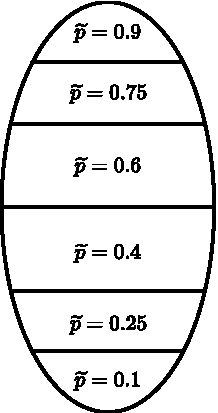
\includegraphics[width=.8\textwidth]{img/partitions}
			\end{center}
		\end{column}
		\begin{column}{0.7\textwidth}

			Let $C = \{c: \mathcal{X} \rightarrow [-1, 1]\}$ be a collection of subsets, generalized as \textbf{real-valued functions}. \pause \newline \\

			$\tilde{p}$ is $(C, \alpha)$-multiaccurate if:
			\begin{gather}
				\max_{c \in C} |\mathbb{E}[c(x)(y-\tilde{p}(x))]| \leq \alpha
			\end{gather} \pause % can c find a pattern in the errors (y-p(x))
			$\tilde{p}$ is $(C, \alpha)$-multicalibrated if:
			\begin{gather}
				\max_{c \in C} \mathbb{E}[|\mathbb{E}[c(x)(y-\tilde{p}(x))]|] \leq \alpha
			\end{gather} \pause
			If we can find correlations with the error, there's some advantage to be gained. We enforce multicalibration to train the \textbf{weak agnostic learner}.
		\end{column}
	\end{columns}
\end{frame}

\begin{frame}{Omnipredictors}
	If we know $p^*$, it is easy for us take take the optimal action. \pause \newline \\

	For $y \in \{0, 1\},~y \sim \text{Bernoulli}(p^*)$. We denote optimal action $t := k_\ell^* \circ p^*$ as post-processing function. \pause \newline \\

	This paper connects multigroup fairness with the notion of a weak agnostic learner, to formulate $(L, C)$-omnipredictors. \pause \newline \\

	\textbf{Intuitively}: the idea is to \textit{extract the predictive power} of the data. \pause \newline \\

	Let $L_{cvx}$ be a set of Lipschitz, convex, bounded losses. \pause If $\tilde{p}$ is $C$-multicalibrated with some error $\alpha$, it is an $(L_{cvx}, C, \alpha)$-omnipredictor. \pause \newline \\

	Multicalibration implies omniprediction for all convex loss functions.
\end{frame}

\begin{frame}{Proof of Optimality}
	As proof for optimality, we evaluate binary classification. Assumptions:
	\begin{enumerate}[label=\arabic*.]
		\item $p^*$ is boolean.
		\item Perfect Mutlicalibration: $\mathbb{E}[c(x)(y^*-v)|\tilde{p}(x)=v]=0,\forall v \in [0, 1], c \in C $
	\end{enumerate} \pause
	\begin{center}
		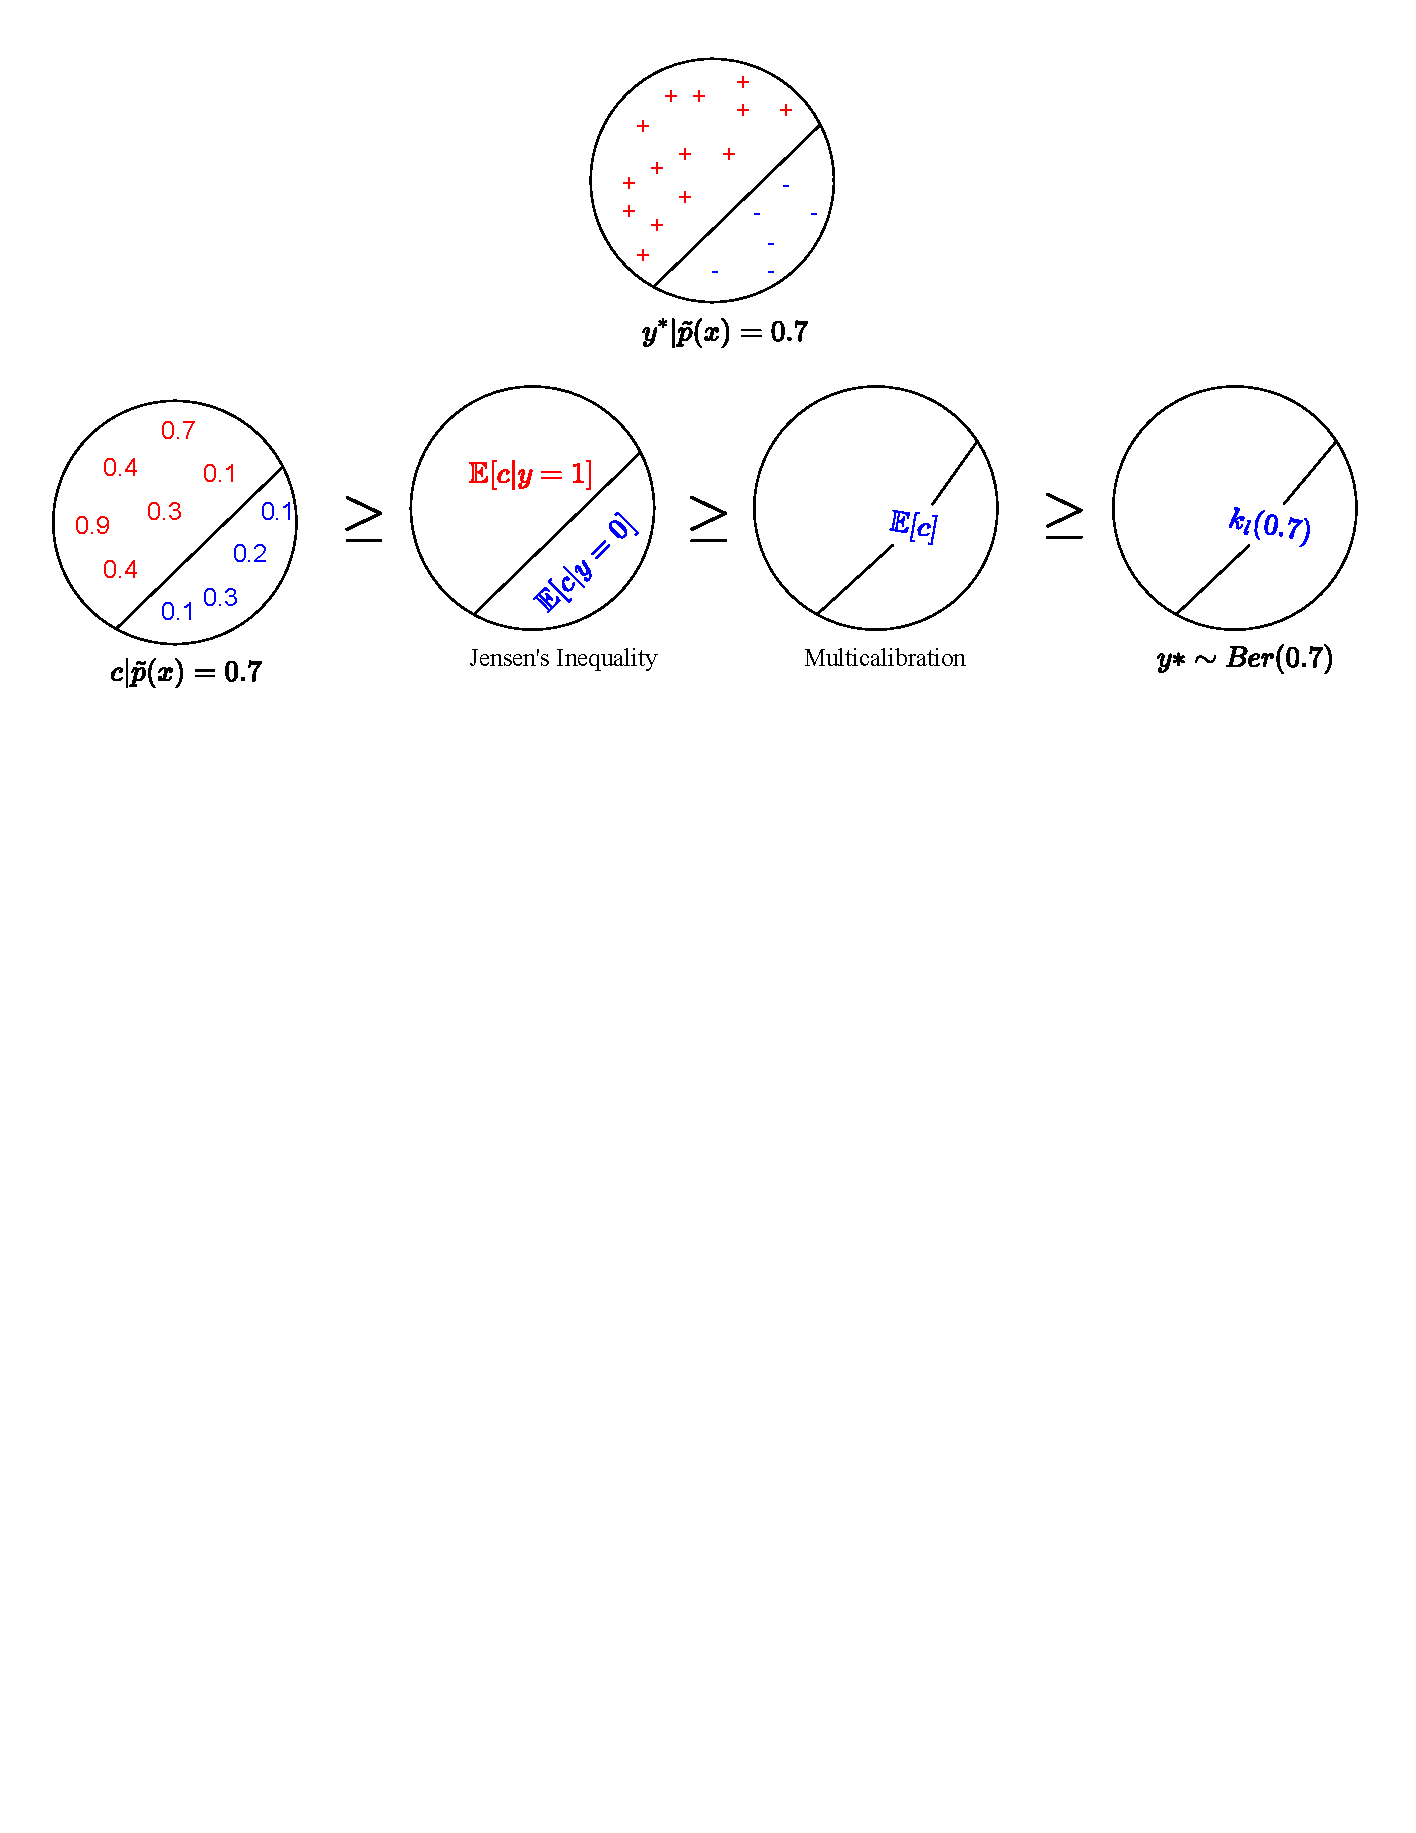
\includegraphics[width=.97\textwidth]{img/proof}
	\end{center}
\end{frame}

\begin{frame}{Training Agnostic Learners} % TODO: fix
	We can train an agnostic learner using the following setup:
	\begin{gather}
		\mathcal{H} : \mathcal{X} \rightarrow \{0, 1\} \\
		\mathcal{D} : \mathcal{X} \times \{0, 1\} \\
		\ell(h \in \mathcal{H}) = \text{Pr}_{(x,y) \sim \mathcal{D}}[h(x) \neq y] = \mathbb{E}_{(x,y) \sim \mathcal{D}}[\ell_1(y, h(x))] \\
		OPT(\mathcal{H}) = \min_{h \in \mathcal{H}} \ell(h)
	\end{gather} \pause
	An agnostic learner for $\mathcal{H}$ produces $f$ s.t. $\ell(f) \leq \text{OPT}(\mathcal{H}) + \epsilon$. \pause \newline \\

	We $(\epsilon, W)$-approximate $\mathcal{H}$ by $\mathcal{C}$ if $\forall h \in \mathcal{H}, \epsilon > 0$, $g_w \in \text{Lin}_{\mathcal{C}}(W)$:
	\begin{gather}
		\mathbb{E}_{(x,y) \sim \mathcal{D}}[|g_w(x) - h(x)|] \leq \epsilon
	\end{gather}

	If partition $\mathcal{S}$ is $\frac{\epsilon}{2W}$-approximately multicalibrated for $\mathcal{C}, \mathcal{D}$, $\ell(h_{\ell_1}^{\mathcal{S}}) \leq \text{OPT}(\mathcal{H}) + \epsilon$ and can identify multicalibrated partitions.
\end{frame}

\begin{frame}{Thank you!}
	\begin{center}
		Have an awesome rest of your day!
	\end{center}
	\begin{center}
		\textbf{Slides:} {\small \url{https://cs.purdue.edu/homes/jsetpal/slides/omnipredictors.pdf}}
	\end{center}
\end{frame}

\end{document}
